\section{An exocentric vision system for Morduc}
\label{sec:concr}
This section will show how to use \textsf{REAR} to implement a 
concrete exocentric vision system, specifically designed for 
Morduc.
%

%
As section \ref{sec:rear} explains, in order to get things 
done, all we need to write is:
\begin{itemize}
\item a concrete subclass of \texttt{Robot}
\item an implementation of the \texttt{IDataLogic} interface
\item an implementation of the \texttt{IImageSelector} interface
\end{itemize}
%
The class diagram of the complete system is reported in figure 
\ref{fig:class_diagram_complete}. 
%
As it's easy to notice, it features two implementations 
of the \texttt{IImageSelector} interface: \texttt{SpacialMetricCalc} 
and \texttt{SweepMetricCalc}. The former is nothing more than 
a mere implementation of the image selection method 2 reported in 
\cite{sugimoto} and already introduced in section \ref{sub:iimageselector}.
%

%
\begin{figure}[!h]
  \begin{center}
    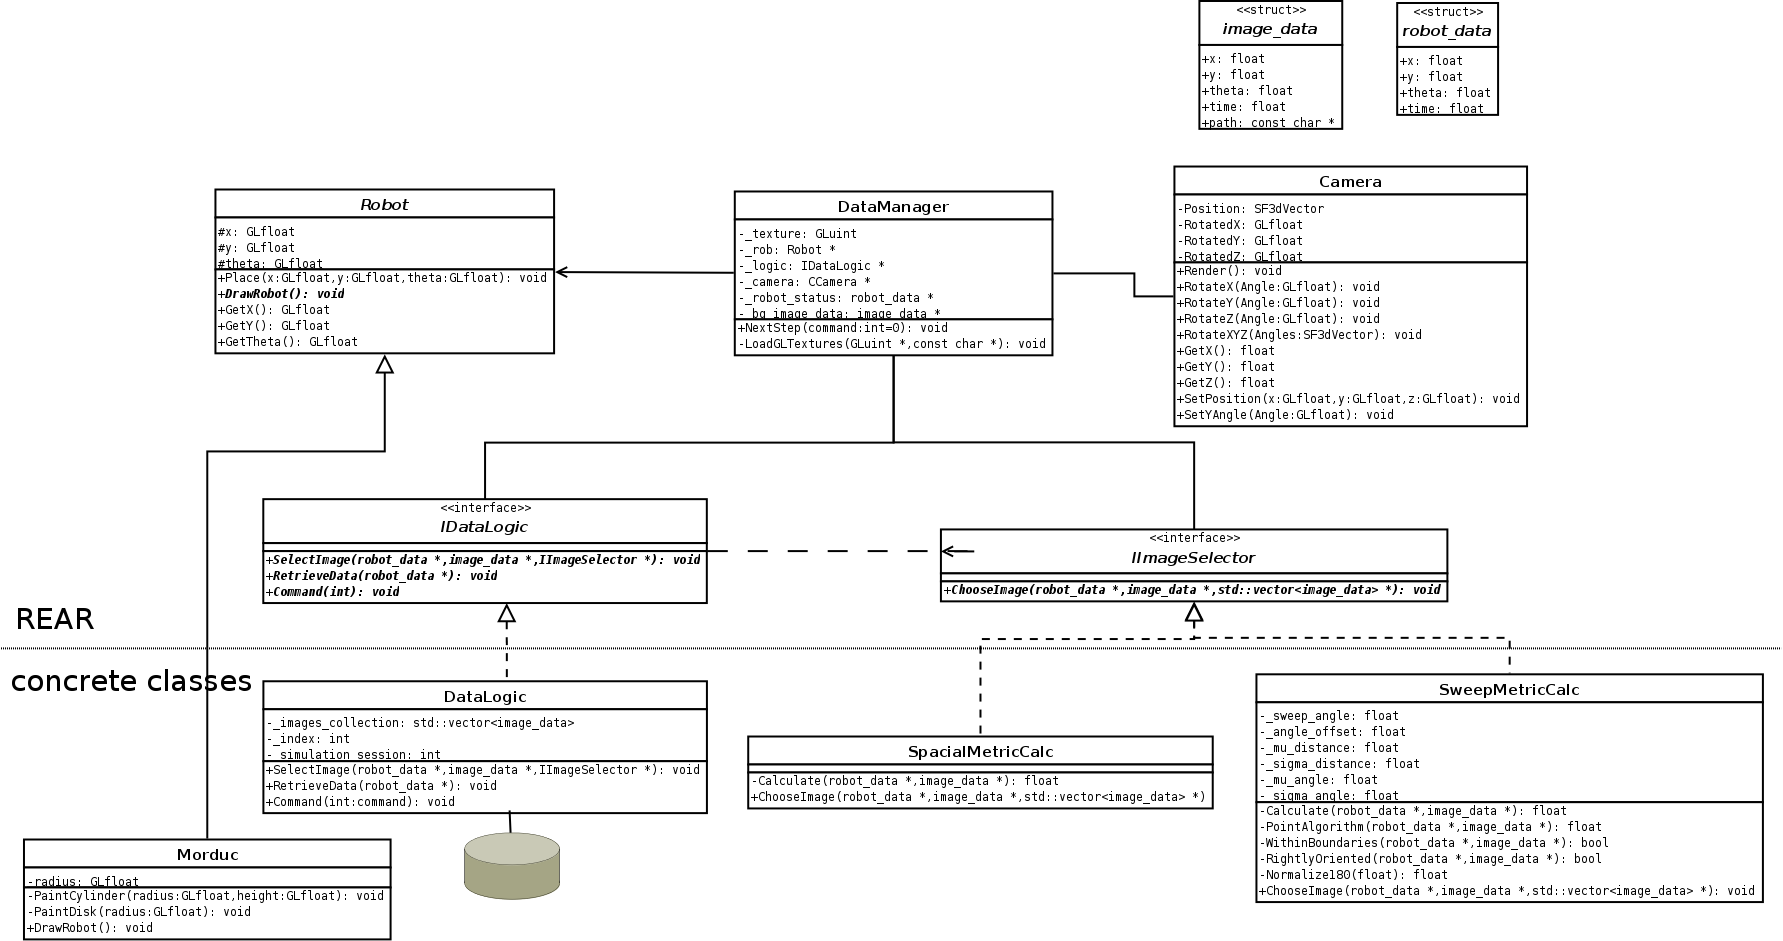
\includegraphics[width=400pt]{img/class_diagram.png} 
    \caption{Class diagram of the whole system}
    \label{fig:class_diagram_complete}
  \end{center}
\end{figure}
%

The latter, instead, encapsulates a brand new selection algorithm. 
It will be widely discussed later in section 
\ref{subsec:sweep_metric_algorithm}.


\subsection{The Morduc Class}
\label{subsec:morducclass}

The \texttt{Morduc} class publicly inherits from \texttt{Robot} 
and, hence, implements the \texttt{DrawRobot()} method:
%
\begin{lstlisting}[caption={\texttt{Morduc} class declaration}, label={code:morducclass}, frame=trBL]
class Morduc : public Robot
{
 private:
  GLfloat radius;
  void PaintCylinder(GLfloat radius,GLfloat height);
  void PaintDisk(GLfloat radius);

 public:
  Morduc(float radius = 4.0f);
  void DrawRobot();
};
\end{lstlisting}
%
Such a method, reported in listing \ref{code:drawrobot}, contains the 
procedure to actually draw the OpenGL model representing Murdoc 
(in reality, Murdoc looks like a stack of three disks linked 
by thin cylinders - see figure \ref{fig:3morduc_opengl}).
%
\begin{lstlisting}[caption={\texttt{Morduc::DrawRobot()} function}, label={code:drawrobot}, frame=trBL]
void Morduc::DrawRobot()
{
  GLfloat reflectance_black[] = { 0.2f, 0.2f, 0.2f};
  GLfloat reflectance_white[] = { 0.8f, 0.8f, 0.8f};
  
  glMatrixMode(GL_MODELVIEW);  
  glPushMatrix();

  // set robot reflectance (it is black)
  glMaterialfv(GL_FRONT_AND_BACK, GL_AMBIENT, 
               reflectance_black);

  // set robot position
  glTranslatef(this -> x, 0.0f, this -> y);

  glRotatef(this -> theta, 0.0f, 1.0f, 0.0f);
  
  // translate on z axis
  // not to make the robot wipe the floor
  glTranslatef(0.0f,0.08f,0.0f);

  glScalef(radius, radius, radius);
  
  // draw robot
  PaintCylinder(1.0f, 0.1);
  PaintDisk(-1.0f);
  glTranslatef(0.0f, 0.1f, 0.0f);
  PaintDisk(1.0f);
  
  glTranslatef(0.0f, 0.6f, 0.0f);

  PaintCylinder(1.0f, 0.1f);
  PaintDisk(-1.0f);
  glTranslatef(0.0f, 0.1f, 0.0f);
  PaintDisk(1.0f);

  glTranslatef(0.8f, 0.0f, 0.0f);
  glColor3f(0.5f, 0.5f, 0.5f);
  PaintCylinder(0.2f, 0.3f);
  glTranslatef(0.0f, 0.3f, 0.0f);
  PaintDisk(0.2f);

  glTranslatef(0,0.401,0);
  glMaterialfv(GL_FRONT_AND_BACK, GL_AMBIENT, 
               reflectance_white);
  PaintDisk(0.1f);
  glTranslatef(0,-0.701,0);
  glMaterialfv(GL_FRONT_AND_BACK, GL_AMBIENT, 
               reflectance_black);

  glTranslatef(-0.8f, 0.0f, 0.0f);
  glColor3f(0.1f, 0.1f, 0.1f);
  glTranslatef(0.0f ,0.6f, 0.0f);
  PaintCylinder(1.0f, 0.1f);
  PaintDisk(-1.0f);
  glTranslatef(0.0f, 0.1f, 0.0f); 
  PaintDisk(1.0f);

  glTranslatef(0.0f, -1.5f, 0.0f);
  glTranslatef(0.0f, 0.0f, 0.8f);
  PaintCylinder(0.1f, 1.5f);
  glTranslatef(0.0f, 0.0f, -1.60f);
  PaintCylinder(0.1f, 1.5f);
  glTranslatef(-0.8f, 0.0f, 0.8f);

  PaintCylinder(0.1f, 1.5f);
  glTranslatef(0.8f, 0.0f, 0.0f);

  glScalef(1/radius, 1/radius, 1/radius);

  glPopMatrix();
}
\end{lstlisting}
%
Notice how such a function implements the skeleton 
presented in listing \ref{code:drawrobot_skeleton}.
%

%
As you have surely noticed, \texttt{Morduc} contains also 
some private attributes, precisely two methods - 
\texttt{PaintCylinder()} and \texttt{PaintDisk()} - and 
a float field - \texttt{radius}.
%
The two methods are just \textit{helper functions}, that is, 
functions that contains a procedure to draw, respectively,  
a \textit{disk} and a \textit{cylinder}.
%
\texttt{radius}, instead, stores the value of the radius 
for the of the cylinders which make up the robot.
%
\begin{figure}[!h]
  \begin{center}
    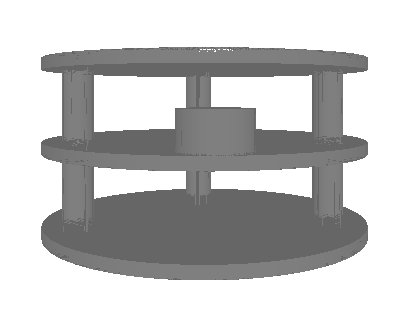
\includegraphics[width=200pt]{img/3morduc_opengl.png}
    \caption{Three dimensional model of Morduc}
    \label{fig:3morduc_opengl}
  \end{center}
\end{figure}
%
After some calibration, the default \texttt{radius} value 
has been set to 4.0.
%

%
\subsection{The DataLogic Class}
\label{sub:datalogic}
For the reasons explained in section \ref{sec:simulator}, 
we used a Morduc simulator in order to generate and record 
test data to use during \textit{offline} tests.
%
For every simulation session, such data consist of:
%
\begin{itemize}
  \item a set of captured images, encoded in the png format
  \item a log file reporting sampled odometry data
\end{itemize}
%
The format of the log file is the one described in section 
\ref{sec:simulator}.
%

%
The concrete \texttt{DataLogic} class will, then, provide 
robot's odometry data and snapshots simply by reading 
those files.
%
Let us have a look at its declaration:
%
\begin{lstlisting}[caption={\texttt{DataLogic} declaration}, label={code:datalogic}, frame=trBL]
class DataLogic : public IDataLogic
{
 private:
  std::vector<image_data> _images_collection;
  int _index;
  int _simulation_session;
  
 public:
  DataLogic(int);
  ~DataLogic();
  void Command(int);
  void RetrieveData(robot_data *);
  void SelectImage(robot_data *, image_data *,
		   IImageSelector *);
};
\end{lstlisting}
%
Upon instantiation, \texttt{DataLogic} objects needs to be 
configured with a session identifier, to be passed to 
the constructor. 
%

%
In order for the \texttt{DataLogic} objects to find them, 
log data must be stored within the relative path 
\texttt{../log}, with respect to the actual execution path.
%
Such a directory must contain a single subdirectory for every 
logged session, named \texttt{log\_$\langle$number of session$\rangle$}. 
%

%
Let us now have a look at how \texttt{DataLogic} implements 
\texttt{IDataLogic} methods:
%
\begin{lstlisting}[caption={\texttt{DataLogic::Command() method}}, label={code:command_method}, frame=trBL]
void DataLogic::Command(int command) 
{

  // sends the command to the robot

  // in our case, just 
  // increase index to point the next line of the file
  _index++;
}
\end{lstlisting}
%
The \texttt{Command()} method is pretty simple in this 
implementation. Since \texttt{DataLogic} has been designed 
for offline testing, there's no actual command to send to the robot.
%
For this reason \texttt{Command()} will not take into account
the received command, the only thing that it does is 
incrementing the private attribute \texttt{\_index}, which 
will be used by \texttt{RetrieveData()} to select which line 
of the log file is to read next.
%
\begin{lstlisting}[caption={\texttt{DataLogic::RetrieveData()} method}, label={code:retrievedata_method}, frame=trBL]
void DataLogic::RetrieveData(robot_data * data)
{
  // pointer to text file containing data
  FILE * position_data;
  char line[50];
  
  std::string * line_read;
  std::string line_values[4];
  std::string position_data_name;
  std::ostringstream o;
  
  int time;
  int line_number = _index;

  // grabbed image metadata
  image_data grabbed_frame_data;
  
  o << "../log/log_" 
    << _simulation_session 
    << "/data_" 
    << _simulation_session << ".txt";

  position_data_name = o.str();

  position_data = fopen(position_data_name.c_str(), "rt");

  while(fgets(line, 50, position_data) &&
	line_number > 1)
    {
      line_number--;
    }

  line_read = new std::string(line);

  std::string buf;
  std::stringstream ss(*line_read);

  // Create vector to hold our words
  std::vector<std::string> tokens;
  
  // put token in vector element
  while (ss >> buf)
    tokens.push_back(buf);

  data->x = atof ( tokens[0].c_str() );
  data->y = atof( tokens[1].c_str() );
  data->theta = TO_DEGREES(- atof ( tokens[2].c_str() ));
  data->time = atof ( tokens[3].c_str() );

  time = (int) data->time;

  // clear the stream and 
  // add a new value to it
  o.str("");
  o.clear();
  o << "../log/log_" 
    << _simulation_session 
    << "/screenshot_" 
    << _simulation_session 
    << "_" << time << ".png";

  // fill grabbed frame metadata
  grabbed_frame_data.x = data->x;
  grabbed_frame_data.y = data->y;
  grabbed_frame_data.theta = data->theta;
  grabbed_frame_data.time = data->time;

  strcpy(grabbed_frame_data.path, o.str().c_str());

  // store the collected metadata 
  // if it's not already stored
  for (std::vector<image_data>::iterator it =
	 _images_collection.begin();
       it != _images_collection.end();
       it++)
    {
      if ( (*it).time == grabbed_frame_data.time )
	{

	  return;
	}
    }

  _images_collection.push_back(grabbed_frame_data);
  return;
}
\end{lstlisting}
%
What the \texttt{RetrieveData()} do is just read the line from the log 
file identified by the \texttt{\_index} private attribute of the class.
Once read, the line is \textit{parsed} and the odometry data contained 
in it is used to fill the \texttt{robot\_data} passed as argument, in 
order to return the \textit{current} robot position.
%
Behind the curtain, \texttt{RetrieveData()} also creates a new 
\texttt{image\_data} structure, fills it with the data just 
gathered and then adds it to the \texttt{\_image\_collection} 
private attribute.
%
This way, every time a new line of the file is read, and, hence, 
every time a new captured image is available, the \texttt{DataLogic} 
is made able to keep track of it using its metadata, without actually 
loading the image - since it would be useless and time-consuming.
%
\begin{lstlisting}[caption={\texttt{DataLogic::SelectImage()} method}, label={code:selectimage_method}, frame=trBL]
void DataLogic::SelectImage(robot_data * robot_status,
                            image_data * bg_image_data,
			    IImageSelector * selector)
{

  // since our data are already stored with vector,
  // we simply pass its reference
  selector -> ChooseImage(robot_status, bg_image_data, &_images_collection);
}
\end{lstlisting}
%
Finally, \texttt{SelectImage()} calls the \texttt{ChooseImage} method 
on an object of type \texttt{IImageSelector}, and passes it, as last 
parameter, a reference to its internal \texttt{\_images\_collection}, 
so that the selector can actually select the image to set as 
background.
%
%
%% \texttt{ChooseImage} takes a pointer to the actual robot status and an
%% \texttt{image\_data} pointer used to return the chosen image, the main difference lies in the third (and last)
%% parameter. The concrete \texttt{ChooseImage} requests an \texttt{std::vector} object with all the image stored,
%% whereas a generic \texttt{IDataLogic} implementation can use a different type of set. In this case, the
%% \texttt{ChooseImage} method must convert the generic set containing \texttt{image\_data} in to an \texttt{std::vector},
%% before calling the \texttt{ChooseImage()} method. Finally, the retrieved image will be then returned.
%
\subsection{Image selection algorithms}
\label{sub:metrics}
As already said, there exists many image selection algorithms. 
Three of them are presented in \cite{sugimoto} and, according 
to the results presented, two proved to be unsatisfactory for 
they do not produced results that could effectively improve 
the quality of the operator-robot interaction.
%
A third one is told to be better but, according to us, it has 
been described poorly and, furthermore, no actual implementation 
of it is given.
%

%
The rest of this chapter will present the theoretical results 
of our investigations on image selection algorithms: 
specifically, it will introduce two algorithms,
which have been implemented by defining two subclasses of 
the \texttt{IImageSelector} interface.
%

%
Both algorithms use a \texttt{Calculate} function to assign a score
value for each image, by knowing the robot status and a single image.
%

%
After assigning a score for every collected image, the one coupled with the
lower score will be returned (or better, assigned to the \texttt{image\_data}
pointer passed to \texttt{ChooseImage} method).
%

%
Moreover, both algorithms take its stand on a specific metric, 
expressed by the \texttt{Calculate}
method.
%

%
In our case, a metric or distance function is a function which defines a
distance between elements belonging to two different and separate sets. The
first one contains the robot status elements, the second one the egocentric images
shot by the robot. Both types of elements are represented, in practice, by two structures
in C++ (see diagram in figure \ref{fig:class_diagram}).
%

%
The \texttt{Calculate} function returns a score (or distance) value associated with a robot
status and a single image. The former is retrieved directly from the \texttt{ChooseImage} 
method, the latter by iterating the image collection parameter.
%

%
Even though the metric function is able to work with every couple of input
data, the two concrete instances of \texttt{IImageSelector} will call
the \texttt{Calculate} method for every stored images, but always with the
same robot status. In this way it is possible to find which is the closer (according to the
chosen metric) image to a specific robot status, by selecting the image coupled with the lowest
score.
%

%
For further details, we refer to chapter \ref{sub:iimageselector}.
%
\subsubsection{The spacial metric algorithm}
\label{subsec:spacial_metric_algorithm}

\begin{figure}[!h]
  \begin{center}
    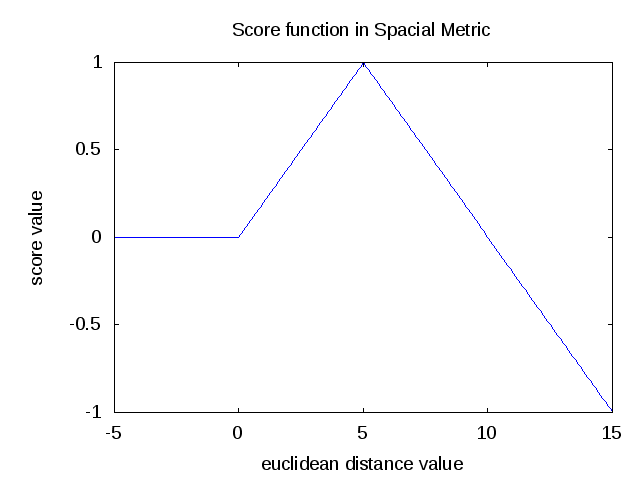
\includegraphics[width=400pt]{img/spacialMetricFunc.png} 
    \caption{Spacial Metric Function}
    \label{fig:spacial_metric_func}
  \end{center}
\end{figure}

This algorithm uses a simple triangle function to couple the image processed with a score.
%

%
The Euclidean distance between robot and image is processed by a triangle function. User specifies
the optimal distance between image and robot, that is the distance value where
the score function returns the maximum tally and therefore where the triangle is centered.
In figure \ref{fig:spacial_metric_func} the optimal distance is set to five.
%

%
Since the \texttt{ChooseImage} method will select the image coupled with the minimum value, we have
to invert the score sign before returning it.
%

%
This algorithm does not care about image orientation. For instance, it could choose an image that
does not include the robot from its point of view. This limit makes the algorithm good only for
quite linear route taken by the robot, but bad for more complex ones. On the other hand, its
implementation is very simple.
%

%
The \texttt{Sweep Metric Algorithm} in chapter \ref{subsec:sweep_metric_algorithm} will try to
go behind this limits.


\subsubsection{The sweep metric algorithm}
\label{subsec:sweep_metric_algorithm}
The "sweep angle" algorithm allows to choose the better background image, in order to implement
the exocentric vision.
%
\begin{figure}[!h]
  \begin{center}
    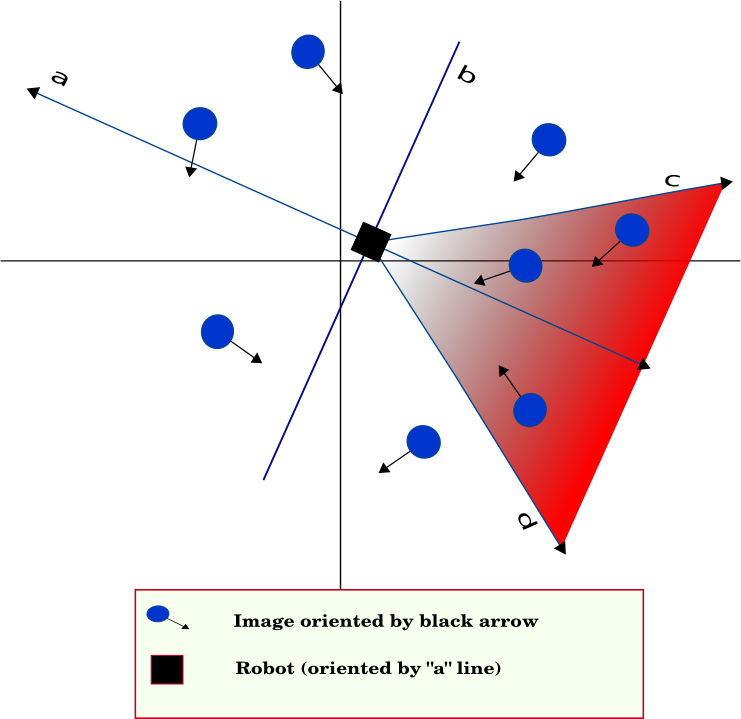
\includegraphics[width=400pt]{img/half_plan_finding.png} 
    \caption{Sweep Angle Algorithm}
    \label{fig:half_plan_finding}
  \end{center}
\end{figure}
%
All the explanation will refer to image \ref{fig:half_plan_finding}. In the latter, the black
square represents the robot, with its orientation indicated by the arrow "a", starting from the
square.
%

%
The several blue circles represent instead the previous shoot images. The orientation of each
image (i.e. the orientation of the robot when they were shoot) is shown by an arrow starting from
each circle.
%

%
We will refer to the line perpendicular to the half line "a" as "b". By rotating clockwise and
counterclockwise the "a" line in the robot centre with a predefined angle (named "sweep angle")
we will obtain the "c" and "d" lines. These define a new portion of the plane (colored with fading red),
named the "sweep area".
%

%
Since we want to control the robot from the rear position, the sought image will be included within
this area: all the other ones will be discarded. Even tough this method allows us to exclude many
images, the selection is certainly not over.
%

%
First of all, we have to discard all the images with an orientation angle that differs too much from the
robot orientation angle. If the difference between the two angles is greater than a specified threshold,
the image can not be chosen as background, because the latter does not include the robot from its point
of view. For instance, if the difference angle between the robot and the image orientation is 180 degrees,
it means that robot and camera are oriented in opposite way, therefore the camera can not see the robot
itself.
%

%
After excluding the badly oriented images, we proceed with the score assignment. The latter is obtained by
the sum of two factors. The first takes in account the image angle orientation: the more the image orientation
angle is close to the robot orientation angle, the more the score is high.
%
\begin{figure}[!h]
  \begin{center}
    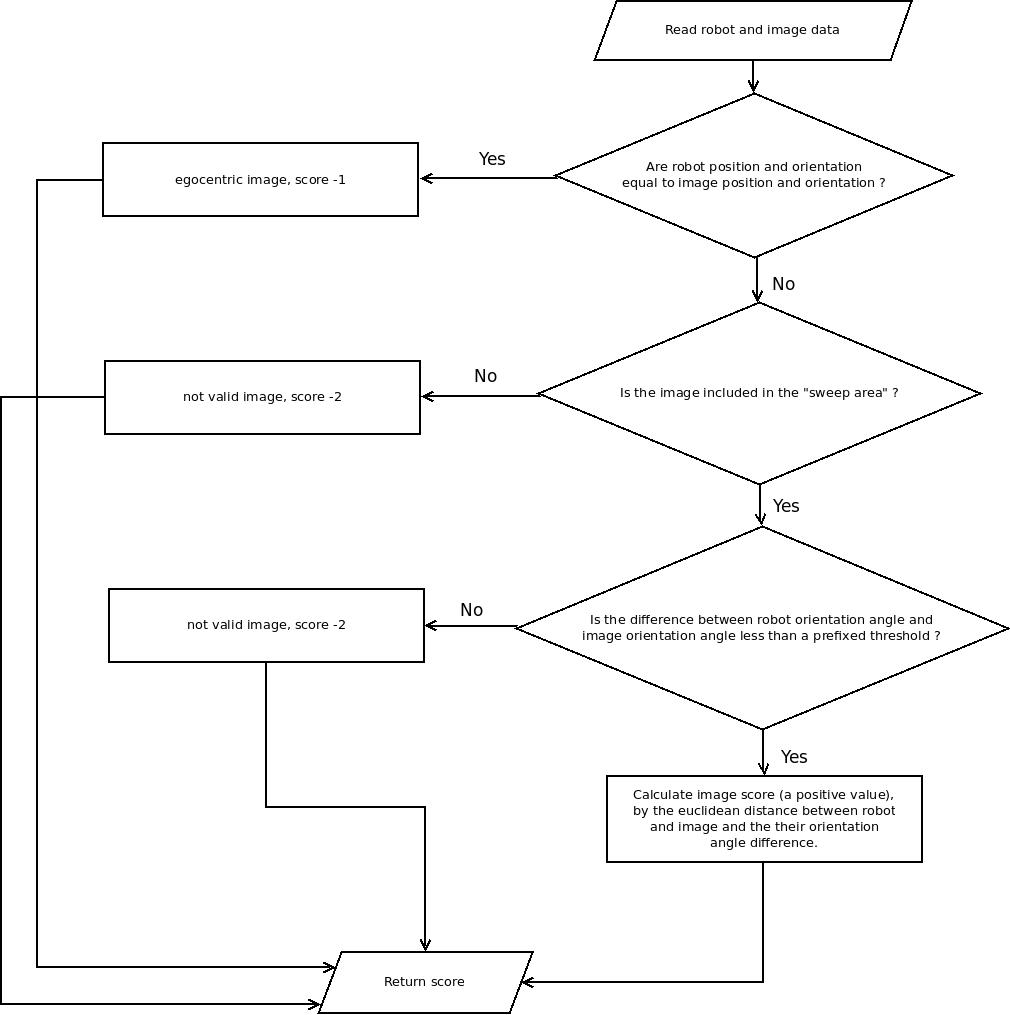
\includegraphics[width=400pt]{img/sweep_angle_diagram.jpeg} 
    \caption{Sweep angle diagram}
    \label{fig:sweep_angle_diagram}
  \end{center}
\end{figure}
%
The function to evaluate the score from the difference between the two angles is a Gaussian function centre
in zero. The return value will be therefore always a positive number.
%

%
The use of a Gaussian function allows to obtain different values even for two very close angle difference
(Gaussian is a injective function), regardless of the assigned variance. Moreover, it is defined for all real
numbers.
In this way is always possible to discern the best angle difference, by choosing the highest value returned by
the function.
%

%
Finally, we have to take in account the Euclidean distance between the image and the robot. If the distance is
zero, we are examining the egocentric image. On one side, the images too close to the robot will be coupled
with a low score, because they are too similar to the egocentric one. On the other side, the images too far
from the robot will be coupled again with a low score, because they would show the robot too distance to
teleguide it properly.
%

%
The preferable image would distance from the robot a predefined quantity, specified by the user. This value
indicate us where to centre another Gaussian function, in order to obtain the score from the distance between
image and robot. The more the image is close to the preferred distance, the more the score assigned will be high.
%

%
The reasons that justifies the use of the Gaussian function are the same previously explained for the angle
difference. The values obtained from the two Gaussian functions, after adding them, form the global score.
%

%
To summarize the method above described (illustrated in figure \ref{fig:sweep_angle_diagram}), we coupled
every image with a score: the one with the maximum value will be chosen and put as background. If the image is
not included in the sweep area (defined by a sweep angle and therefore by the "c" and "d" line) it has to be
discarded. The score assigned will be -2.
%

%
The images situated within the sweep area, but with an orientation angle that differs too much from the robot
orientation angle, have to be discarded as the previous one: the score assigned will be -2 again.
If the image position and orientation coincide with robot position and orientation, the image represents the
egocentric vision. We remember that in our set there will always be the egocentric image, and that this will be
choose as background when no other image for exocentric vision are available. The score coupled with the egocentric 
vision will be -1.
%

%
Finally, all the other images - if present - are coupled with a positive number, because obtained by the sum of
values calculated with Gaussian functions. The most high score indicate the better image to chose as background;
if there are no preferable images, the image with -1 (i.e. the egocentric image) will be chosen.
%

%
Because the \texttt{ChooseImage} method is designed to choose the image with the minimum score and not with maximum,
all we have to do is multiply every score for -1 before returning it: in this way we convert a maximum research in
a minimum one.
%

%
\paragraph{The WithinBoundaries algorithm}
\label{par:withinboundaries}

Checking if an image is included in the "sweep angle" (see chapter \ref{subsec:sweep_metric_algorithm} for its
definition) could be something not too easy to implement. Given image coordinates, robot coordinates and robot
orientation, the \texttt{WithinBoundaries} method must replays (with a true or false response) to the question
"is the image included in the sweep area ?", shown in previous diagram (figure \ref{fig:sweep_angle_diagram}).
%

%
Since the area defined by the "sweep angle" depends on robot coordinates and orientation, we should insert in
the source code a lot of geometrical and mathematical rules, frequently not immediately comprehensible
(even for the authors). For this reason we decided to use a different approach.
%

\begin{figure}[htp]
  \begin{center}
    \subfigure[Initial robot and image coordinates]{
      \label{fig:sweepal_start}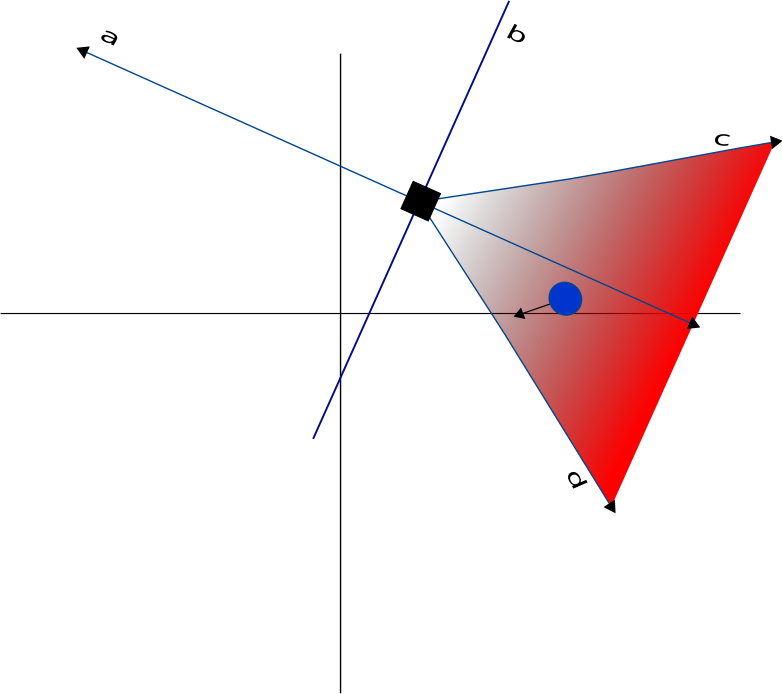
\includegraphics[width=175pt, height=175pt]{img/sweepal_start.png}
    }
    \hspace*{15pt}
    \subfigure[Translated system]{
      \label{fig:sweepal_translate}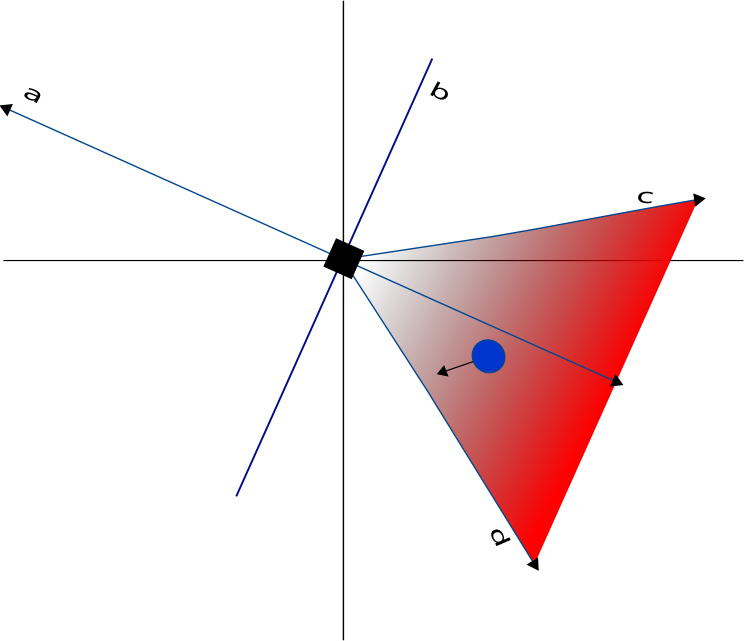
\includegraphics[width=175pt, height=175pt]{img/sweepal_translate.png}
    }

    \subfigure[Rotated system]{
      \label{fig:sweepal_rotate}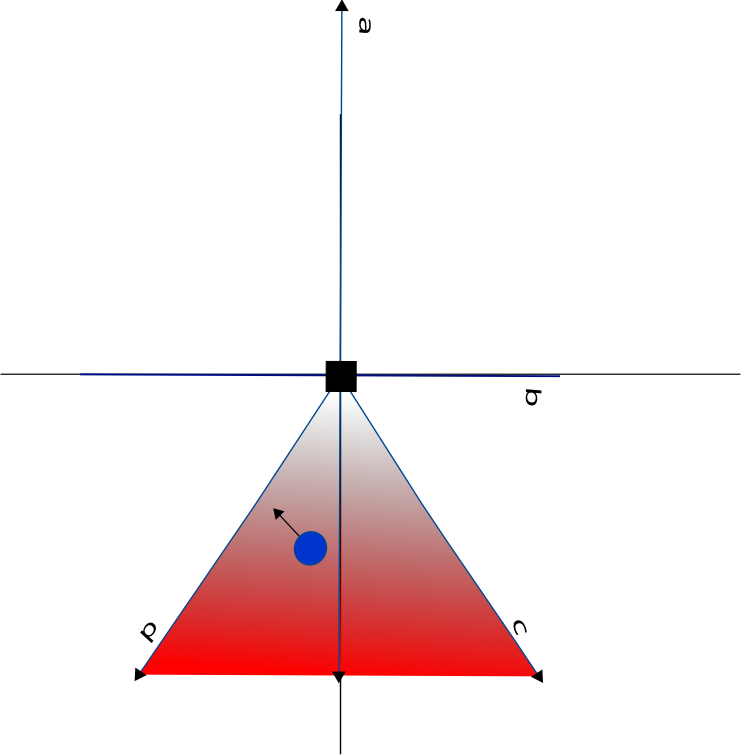
\includegraphics[width=175pt, height=175pt]{img/sweepal_rotate.png}
    } 
    \hspace*{15pt}
    \subfigure[Triangle AOB]{
      \label{fig:sweepal_triangle}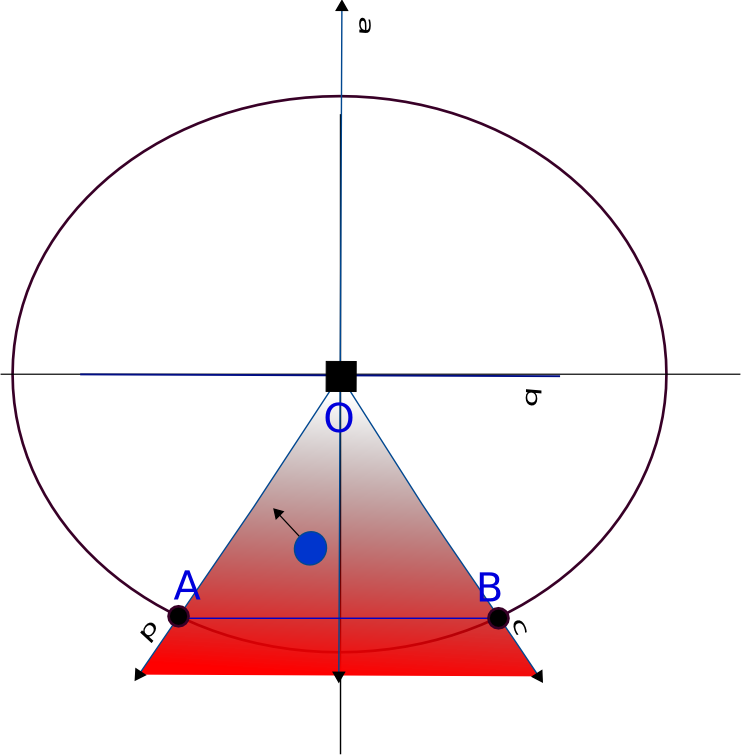
\includegraphics[width=175pt, height=175pt]{img/sweepal_triangle.png}
    } 

    \vspace*{20pt}
    \subfigure[Symbol definition]{
      \label{fig:sweepal_caption}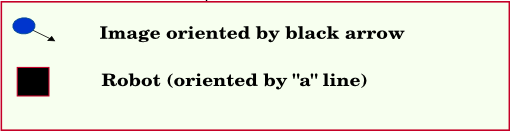
\includegraphics[width=255pt, height=65pt]{img/sweepal_caption.png}
    } 

  \end{center}
  \caption{WithinBoundaries algorithm}
  \label{fig:withingboundaries}
\end{figure}

%
Before checking if a point (i.e. an image) is included in the "sweep angle", the robot and image coordinates
are translated and then rotated, in order to move the robot in the origin of the axis and to overlap its
orientation arrow with the y-axis. The two transformations are shown in figure \ref{fig:sweepal_translate} and
\ref{fig:sweepal_rotate}, while the robot and image starting coordinates are shown in figure \ref{fig:sweepal_start}.
%

%
After executing these transformations, the sweep area is always situated in the second and third quadrant, as
shown in figure \ref{fig:sweepal_rotate}. Now the "c" and "d" lines pass both from the origin. For an exhaustive
definition of line "c" and "d" see chapter \ref{subsec:sweep_metric_algorithm}.
%

%
If we draw a circle centered in the axis origin, the intersection between the circle and the "c" and "d" lines will
return four points in the plan. Among these, the points situated in the second and third quadrant define a triangle
with the centre of the XY axis: this will be our "sweep area", where to check if an image is included or not. Note
that we choose the points with negative Y value (named "A" and "B") due to the translation and rotation operated
before. Again, see figure \ref{fig:sweepal_triangle} for a graphical example.
%

%
The circle radius must be a value large enough to include a wide number of images. In our case we defined it with a
value of five hundred, in order to reduce the difference between the abstract "sweep area" and the practical triangle
"AOB" (figure \ref{fig:sweepal_triangle}) used to simplify the algorithm.
%

%
Defined the "AOB" triangle, we have to cope with a well-known problem: checking if a point is included or not in a
triangle. The better (and more rapid) way to resolve the problem exploits the cross product between vectors
in three-dimensional Euclidean space.
%

%
\begin{figure}[!h]
  \begin{center}
    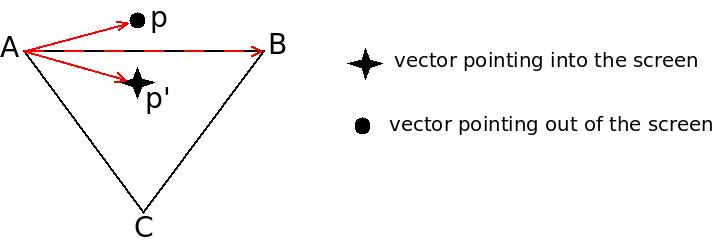
\includegraphics[width=300pt]{img/sweepal_crossproductABC.jpeg} 
    \caption{Cross product between vectors}
    \label{fig:sweepal_crossproductABC}
  \end{center}
\end{figure}
%

Referring to the image \ref{fig:sweepal_crossproductABC}, the cross product of [A-B] and [A-p] will result a vector
pointing out of the screen. On the other hand, the cross product of [A-B] and [A-p'] will result a vector pointing
into the screen.
%

%
The cross product of [A-B] with the vector from A to any point above the segment AB turns out with a resulting vector
points out of the screen, while using any point below AB yields with a vector pointing into the screen. We have to
distinguish which direction a resulting vector must have in order to consider the point "p" inside the triangle.
%

%
Because the triangle can be oriented in any way, what we need is a reference point, that is a point that we know is
on a certain side of the line. For our triangle (figure \ref{fig:sweepal_crossproductABC}), this is just the third
point C.
%

%
Any point "p", where [A-B] cross [A-p] does not point in the same direction as [A-B] cross [A-C], is not inside the
triangle. If the cross products do point in the same direction, then we need to test "p" with the other lines as well.
If the point was on the same side of AB segment as C, and is also on the same side of BC segment as A, and on the same
side of CA segment as B, then it is in the triangle.
%

%
The chief disadvantage regarding the approach above described is that the sweep angle value must be strictly greater
than zero and strictly less than ninety degrees. If the sweep angle exceeds previous limits the algorithm will executes
with a wrong triangle AOB (we remember that AOB angle, shown in figure \ref{fig:sweepal_triangle}, is equal to twice
the sweep angle).
%

%
The described procedure, whose aim is knowing if a point is included within a triangle, can be found in reference
\cite{withinboundaries:pointintriangle}. Its result is in the end the sought answer to the beginning question "is the
image included in the sweep area ?" (figure \ref{fig:sweep_angle_diagram}) and will be returned by the
\texttt{WithinBoundaries} method by means of a boolean value.
%
